\documentclass[aspectratio=169, table, 12pt]{beamer}

% Preamble bersama seluruh slide mata kuliah ini.
% Dipanggil dari slides/sessionXX/sessionXX.tex tepat sesudah baris
% \documentclass[aspectratio=169, table, 12pt]{beamer}
% Paket tambahan yang hanya dibutuhkan satu sesi ditulis di berkas sesi itu.

\usepackage{colortbl}
\usepackage{xcolor}
\usepackage{listings}
\usepackage{tabularx}
\usepackage{booktabs}
\usepackage{tikz}
\usepackage{pgfplots}
\pgfplotsset{compat=1.18}
\usetikzlibrary{arrows.meta, positioning, calc, fit, shapes.geometric,
	shapes.multipart, backgrounds, matrix, chains, trees}

\makeatletter
\def\input@path{{../theme/}}
\makeatother
\graphicspath{{../theme/}{../../figures/}}
\usetheme{Pradita}

\definecolor{praditagreen}{RGB}{37, 113, 71}

% Tema membuat garis tabel berwarna putih. Dikembalikan agar tabel terbaca.
\arrayrulecolor{black}
\setlength{\arrayrulewidth}{0.5pt}

\lstdefinelanguage{yaml}{
	basicstyle=\ttfamily\scriptsize,
	keywordstyle=\color{blue}\bfseries,
	commentstyle=\color{gray}\itshape,
	stringstyle=\color{red},
	showstringspaces=false,
	breaklines=true,
	frame=lines,
	numbers=none,
	backgroundcolor=\color{lightgray!10},
	tabsize=2,
	morecomment=[l]{\#}
}

\lstdefinelanguage{json}{
	basicstyle=\ttfamily\scriptsize,
	stringstyle=\color{red},
	commentstyle=\color{gray},
	breaklines=true,
	showstringspaces=false,
	tabsize=2,
	numbers=none,
	frame=lines,
	backgroundcolor=\color{lightgray!10},
	string=[s]{"}{"}
}

\lstdefinelanguage{bash}{
	keywords={},
	basicstyle=\ttfamily\scriptsize,
	ndkeywords={docker, kubectl, helm, curl, git, terraform},
	ndkeywordstyle=\color{purple}\bfseries,
	sensitive=true,
	commentstyle=\color{gray},
	numbers=none,
	breaklines=true,
	frame=lines,
	backgroundcolor=\color{lightgray!10},
	tabsize=2,
	comment=[l]{\#},
	showstringspaces=false
}

\lstdefinelanguage{http}{
	keywords={GET, POST, PUT, PATCH, DELETE, HEAD, OPTIONS, HTTP},
	basicstyle=\ttfamily\scriptsize,
	keywordstyle=\color{blue}\bfseries,
	sensitive=true,
	numbers=none,
	breaklines=true,
	frame=lines,
	backgroundcolor=\color{lightgray!10},
	tabsize=2,
	showstringspaces=false
}

\subtitle{IT40713 · Cloud-Native \& Microservices Architecture}
\author{\textbf{Alfa Yohannis}}


\title{\Huge Komunikasi Layanan\\ \vspace{10pt} dan Event-Driven}

\begin{document}

\frame{\titlepage}

\begin{frame}
  \frametitle{Isi Pertemuan}
  \vspace{14pt}
  \begin{columns}[t]
    \column{0.5\textwidth}
    {\small\tableofcontents[sections={1-4}]}

    \column{0.5\textwidth}
    {\small\tableofcontents[sections={5-8}]}
  \end{columns}
\end{frame}

\begin{frame}{\hfill}
  \centering
  \Huge{\textbf{Mengapa notifikasi yang\\mati membuat pasien\\gagal membuat janji?}}
\end{frame}

\section{Tujuan dan Konteks}

\begin{frame}{\hfill}
  \centering
  \Huge{\textbf{Tujuan dan Konteks}}
\end{frame}

\begin{frame}{{\Large Tujuan Pembelajaran}}
  \vspace{10pt}
  \begin{itemize}
    \item Membedakan komunikasi sinkron dan asinkron beserta dampaknya terhadap
          ketersediaan layanan.
    \item Memodelkan proses bisnis sebagai rangkaian \textit{event}.
    \item Membandingkan koordinasi berbasis \textit{choreography} dan
          \textit{orchestration}.
  \end{itemize}
\end{frame}

\begin{frame}{{\Large Insiden Notifikasi Medikara+, Maret 2026}}
  \vspace{6pt}
  \begin{itemize}
    \item Layanan WhatsApp milik vendor notifikasi terganggu tiga jam.
    \item Jam sibuk 07.00 sampai 10.00: sekitar 175 janji temu per jam.
    \item Sekitar 520 janji temu gagal dibuat; pusat panggilan kewalahan.
    \item Penyebab: Medikara+ menunggu empat sistem secara berurutan.
    \item Pola yang sama ada di integrasi \textit{point-to-point} SIMRS, ERP,
          BPJS Kesehatan, dan SATUSEHAT.
  \end{itemize}
\end{frame}

\begin{frame}{{\Large Diagram Konsep Bab 9}}
  \centering
  {\small\bfseries Penyampaian event dan penanganan duplikasi}\par\medskip
  \adjustbox{width=0.96\textwidth,height=0.7\textheight,keepaspectratio}{%
    % Diagram konsep Bab 9: Penyampaian event dan penanganan duplikasi.
% Dibangkitkan tools/render-diagrams.py dari figures/chapter-diagrams.json;
% ubah data JSON lalu jalankan ulang skrip, jangan sunting berkas ini langsung.
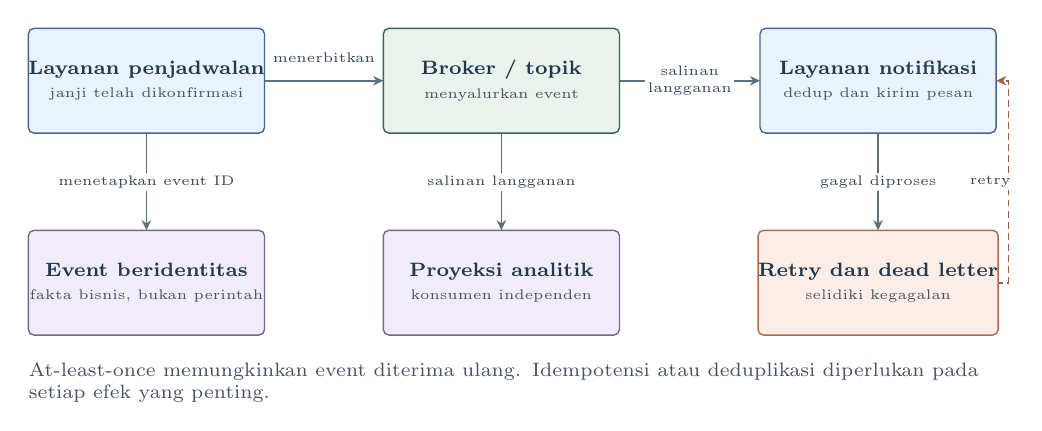
\begin{tikzpicture}[
  x=0.92cm, y=0.95cm,
  kotak konsep/.style={draw, line width=0.5pt, rounded corners=2pt,
    align=center, minimum width=2.999cm,
    minimum height=1.330cm, inner sep=0pt, font=\scriptsize,
    text=konsepJudul},
  peran actor/.style={kotak konsep, fill=konsepIsiActor, draw=konsepGarisActor},
  peran service/.style={kotak konsep, fill=konsepIsiService, draw=konsepGarisService},
  peran control/.style={kotak konsep, fill=konsepIsiControl, draw=konsepGarisControl},
  peran data/.style={kotak konsep, fill=konsepIsiData, draw=konsepGarisData},
  peran outcome/.style={kotak konsep, fill=konsepIsiOutcome, draw=konsepGarisOutcome},
  peran risk/.style={kotak konsep, fill=konsepIsiRisk, draw=konsepGarisRisk},
  panah konsep/.style={-{Stealth[length=1.3mm, width=1.2mm]}, line width=0.6pt,
    draw=konsepPanah},
  panah putus/.style={panah konsep, draw=konsepPanahPutus,
    dash pattern=on 2.5pt off 1.5pt},
  label panah/.style={font=\tiny, align=center, fill=white,
    inner sep=1pt, text=konsepLabel},
  catatan/.style={font=\scriptsize, align=left, anchor=north west,
    inner sep=0pt, text width=12.291cm, text=konsepTeks,
    execute at begin node={\hyphenpenalty=10000\hbadness=10000\relax}},
]
  \definecolor{konsepIsiActor}{HTML}{EEF1F6}
  \definecolor{konsepGarisActor}{HTML}{50627D}
  \definecolor{konsepIsiService}{HTML}{EAF2FB}
  \definecolor{konsepGarisService}{HTML}{3F6893}
  \definecolor{konsepIsiControl}{HTML}{E9F3EC}
  \definecolor{konsepGarisControl}{HTML}{316B4B}
  \definecolor{konsepIsiData}{HTML}{F1EDF8}
  \definecolor{konsepGarisData}{HTML}{786394}
  \definecolor{konsepIsiOutcome}{HTML}{E4F2EC}
  \definecolor{konsepGarisOutcome}{HTML}{236C57}
  \definecolor{konsepIsiRisk}{HTML}{FCEDE7}
  \definecolor{konsepGarisRisk}{HTML}{B36947}
  \definecolor{konsepJudul}{HTML}{20394F}
  \definecolor{konsepTeks}{HTML}{455264}
  \definecolor{konsepLabel}{HTML}{35485C}
  \definecolor{konsepPanah}{HTML}{5C7084}
  \definecolor{konsepPanahPutus}{HTML}{A15D40}
  % Panah dan label lebih dahulu; kotak menutupi sisa latar label.
  \draw[panah konsep] (0.93,0) -- (2.57,0);
  \draw[panah konsep] (5.83,0) -- (7.77,0);
  \draw[panah konsep] (-0.7,-0.7) -- (-0.7,-2);
  \draw[panah konsep] (4.2,-0.7) -- (4.2,-2);
  \draw[panah konsep] (9.4,-0.7) -- (9.4,-2);
  \draw[panah putus] (11.03,-2.7) -- (11.2,-2.7) -- (11.2,0) -- (11.03,0);
  \node[label panah] at (1.75,0.31) {menerbitkan};
  \node[label panah] at (6.8,0) {salinan\\langganan};
  \node[label panah] at (-0.7,-1.35) {menetapkan event ID};
  \node[label panah] at (4.2,-1.35) {salinan langganan};
  \node[label panah] at (9.4,-1.35) {gagal diproses};
  \node[label panah] at (10.95,-1.35) {retry};
  \node[peran service] (prod) at (-0.7,0)
    {\textbf{Layanan penjadwalan}\\[0.5pt]{\tiny\color{konsepTeks}janji telah dikonfirmasi}};
  \node[peran control] (broker) at (4.2,0)
    {\textbf{Broker / topik}\\[0.5pt]{\tiny\color{konsepTeks}menyalurkan event}};
  \node[peran service] (notif) at (9.4,0)
    {\textbf{Layanan notifikasi}\\[0.5pt]{\tiny\color{konsepTeks}dedup dan kirim pesan}};
  \node[peran data] (event) at (-0.7,-2.7)
    {\textbf{Event beridentitas}\\[0.5pt]{\tiny\color{konsepTeks}fakta bisnis, bukan perintah}};
  \node[peran data] (analis) at (4.2,-2.7)
    {\textbf{Proyeksi analitik}\\[0.5pt]{\tiny\color{konsepTeks}konsumen independen}};
  \node[peran risk] (retry) at (9.4,-2.7)
    {\textbf{Retry dan dead letter}\\[0.5pt]{\tiny\color{konsepTeks}selidiki kegagalan}};
  \node[catatan] at (-2.33,-3.77)
    {At-least-once memungkinkan event diterima ulang. Idempotensi atau deduplikasi diperlukan pada setiap efek yang penting.};
\end{tikzpicture}
}
\end{frame}

\section{Sinkron dan Asinkron}

\begin{frame}{\hfill}
  \centering
  \Huge{\textbf{Sinkron dan Asinkron}}
\end{frame}

\begin{frame}{{\Large Sinkron dan Asinkron}}
  \footnotesize
  \begin{tabularx}{\textwidth}{>{\raggedright\arraybackslash}p{2.8cm}
      >{\raggedright\arraybackslash}X >{\raggedright\arraybackslash}X}
    \hline
    \textbf{Aspek} & \textbf{Sinkron (\textit{request/response})}
      & \textbf{Asinkron (lewat pesan)} \\
    \hline
    Cara kerja & Pemanggil menunggu jawaban & Pesan dititipkan, pengirim lanjut \\
    \hline
    Syarat & Semua pihak hidup bersamaan & Pengirim dan perantara hidup \\
    \hline
    Waktu tunggu & Jumlah semua panggilan & Hanya waktu menitipkan pesan \\
    \hline
    Wujud gagal & Pengguna melihat pesan gagal & Pesan menumpuk, hasil terlambat \\
    \hline
    Cocok untuk & Jawaban yang dibutuhkan saat itu & Pekerjaan yang boleh terlambat \\
    \hline
  \end{tabularx}

  \vspace{10pt}
  \small
  Analogi: menelepon gudang dan menunggu di gagang, atau meninggalkan memo di
  kotak masuknya.
\end{frame}

\begin{frame}{{\Large Rantai Sinkron dan Ketersediaan}}
  \vspace{6pt}
  \begin{itemize}
    \item Ketersediaan gabungan rantai = hasil kali ketersediaan tiap mata
          rantai.
    \item Waktu tunggu tiap panggilan dijumlahkan.
    \item Empat sistem 99,5 persen: alur sekitar 98 persen, sekitar 14 jam
          gagal per bulan.
    \item Pemilik alur ikut menanggung gangguan sistem yang tidak dimilikinya.
    \item Slot jadwal dokter: sinkron. Pengingat kontrol (1.400 per hari):
          cukup asinkron.
  \end{itemize}
\end{frame}

\begin{frame}{{\Large Alur Janji Temu: Sebelum dan Sesudah}}
  \centering
  \eadiagram{../../figures/ch09-rantai-sinkron.tex}
\end{frame}

\begin{frame}{{\Large Kasus Medikara: Alur Janji Temu}}
  \vspace{6pt}
  \begin{itemize}
    \item Sekarang: 99,9 $\times$ 99,0 $\times$ 99,5 $\times$ 99,0 persen
          $\approx$ 97,4 persen, sekitar 18,6 jam gagal per bulan.
    \item Waktu tunggu 150 + 1.200 + 400 + 650 milidetik $\approx$ 2,4 detik.
    \item Rancangan ulang: hanya jadwal dokter dan \textit{broker} (99,95
          persen) yang ditunggu.
    \item Hasilnya sekitar 99,85 persen (65 menit per bulan) dan 170 milidetik.
    \item Harganya: pasien BPJS bisa berstatus "perlu konfirmasi penjamin",
          diputuskan bagian pelayanan.
  \end{itemize}
\end{frame}

\section{Antrean dan Publish/Subscribe}

\begin{frame}{\hfill}
  \centering
  \Huge{\textbf{Antrean dan\\Publish/Subscribe}}
\end{frame}

\begin{frame}{{\Large Antrean Pesan dan Publish/Subscribe}}
  \centering
  \eadiagram{../../figures/ch09-antrean-pubsub.tex}

  \vspace{6pt}
  \small
  Analogi: nomor antrean di bank dan papan pengumuman RT.
\end{frame}

\begin{frame}{{\Large Peran Event Broker}}
  \vspace{6pt}
  \begin{itemize}
    \item \textit{Broker} menerima, menyimpan, dan mengantar pesan kepada
          penerima yang berhak.
    \item Antrean: satu pesan untuk satu penerima; penerima berbagi beban.
    \item \textit{Publish/subscribe}: tiap pelanggan mendapat salinan.
    \item Pengingat naik dari 1.400 ke 4.000 per hari: cukup tambah pengirim.
    \item Integrasi \textit{point-to-point} baru sekitar enam minggu; pelanggan
          topik baru cukup mendaftar.
  \end{itemize}
\end{frame}

\begin{frame}{{\Large Gambaran Produk Broker}}
  \footnotesize
  \begin{tabularx}{\textwidth}{>{\raggedright\arraybackslash}p{3.6cm}
      >{\raggedright\arraybackslash}X >{\raggedright\arraybackslash}X}
    \hline
    \textbf{Produk} & \textbf{Sifat utama} & \textbf{Cocok untuk} \\
    \hline
    RabbitMQ & Antrean dan topik; pesan dihapus setelah diakui
      & Pembagian kerja, aturan rute luwes \\
    \hline
    Apache Kafka & Log \textit{event} dengan masa retensi; bisa dibaca ulang
      & Volume besar, analitik, baca riwayat \\
    \hline
    Antrean terkelola (SQS, Service Bus) & Penyedia mengurus server
      & Tim kecil tanpa operasi \textit{broker} \\
    \hline
    \textit{Pub/sub} terkelola (Pub/Sub, SNS, Event Grid) & Topik terkelola
      & Penyebaran \textit{event} dalam satu penyedia \\
    \hline
  \end{tabularx}

  \vspace{10pt}
  \small
  \textit{Broker} ikut menyimpan isi pesan: aturan lokasi data (Bab 2) berlaku.
\end{frame}

\begin{frame}{{\Large Pendalaman: Broker Lokal (Opsional)}}
  \vspace{4pt}
  \small
  \begin{enumerate}
    \item Folder \berkas{sources/chapter09/contoh-broker-lokal}.
    \item \texttt{docker compose up -d}, lalu \texttt{pip install pika}.
    \item \texttt{python kirim\_terima\_event.py kirim}: \textit{event} yang
          sama terkirim dua kali.
    \item Konsol \url{http://localhost:15672}: antrean berisi dua pesan.
    \item \texttt{python kirim\_terima\_event.py terima}: pesan kedua dilewati.
  \end{enumerate}
  \vspace{4pt}
  {\footnotesize Hanya di komputer sendiri; port tidak dibuka ke jaringan
  publik.}
\end{frame}

\section{Pola Event}

\begin{frame}{\hfill}
  \centering
  \Huge{\textbf{Pola Event}}
\end{frame}

\begin{frame}{{\Large Event dan Perintah}}
  \vspace{6pt}
  \begin{itemize}
    \item \textit{Event}: fakta bisnis dalam bentuk lampau, satu pemilik,
          tidak dapat dibatalkan.
    \item \textit{Event}: \texttt{JanjiTemuDibuat}; penerbit tidak peduli siapa
          yang bereaksi.
    \item Perintah: \texttt{KirimPengingat}; untuk penerima tertentu yang boleh
          menolak.
    \item Waspadai \textit{event} yang menjadi perintah terselubung.
    \item Nama dari \textit{ubiquitous language} dan papan EventStorming Bab 6.
  \end{itemize}
\end{frame}

\begin{frame}{{\Large Tiga Pola Event}}
  \scriptsize
  \begin{tabularx}{\textwidth}{>{\raggedright\arraybackslash}p{2.6cm}
      >{\raggedright\arraybackslash}X >{\raggedright\arraybackslash}X
      >{\raggedright\arraybackslash}X}
    \hline
    \textbf{Pola} & \textbf{Isi \textit{event}} & \textbf{Kelebihan}
      & \textbf{Biaya} \\
    \hline
    \textit{Event notification} & Kabar singkat dan nomor rujukan
      & Keterkaitan rendah; data sensitif tetap di pemilik
      & Alur tersebar; panggilan balik \\
    \hline
    \textit{Event-carried state transfer} & Data yang berubah
      & Penerima mandiri; waktu tunggu pendek
      & Data tersalin; data pribadi menyebar \\
    \hline
    \textit{Event sourcing} & Seluruh perubahan status
      & Jejak audit lengkap & Rumit; perubahan bentuk \textit{event} \\
    \hline
  \end{tabularx}

  \vspace{10pt}
  \small
  Analogi: notifikasi bank "cek aplikasi", pesan mutasi lengkap, dan buku
  tabungan.
\end{frame}

\begin{frame}{{\Large Kasus Medikara: Tiga Event Pertama}}
  \scriptsize
  \begin{tabularx}{\textwidth}{>{\raggedright\arraybackslash}p{3.0cm}
      >{\raggedright\arraybackslash}p{2.3cm} >{\raggedright\arraybackslash}X
      >{\raggedright\arraybackslash}X r}
    \hline
    \textbf{\textit{Event}} & \textbf{Pola} & \textbf{Isi data}
      & \textbf{Pelanggan} & \textbf{Per hari} \\
    \hline
    \texttt{JanjiTemuDibuat} & \textit{Notification} plus sebagian data
      & Nomor janji, rujukan pasien, waktu & Notifikasi, pendaftaran,
      kepesertaan, analitik & 1.400 \\
    \hline
    \texttt{HasilLabTersedia} & \textit{Notification} murni
      & Nomor permintaan, penanda kritis & Pelayanan klinis, notifikasi,
      penagihan & 2.600 \\
    \hline
    \texttt{TagihanTerbit} & \textit{State transfer}
      & Nomor tagihan, total, penjamin & Notifikasi, ERP, klaim & 3.300 \\
    \hline
  \end{tabularx}

  \vspace{8pt}
  \small
  Isi hasil laboratorium tidak ikut tersebar: jawaban atas temuan audit
  kontrol akses.
\end{frame}

\begin{frame}{{\Large Pendalaman: CloudEvents dan AsyncAPI}}
  \vspace{6pt}
  \begin{itemize}
    \item CloudEvents 1.0.2: format data \textit{event} netral vendor,
          \textit{graduated} di CNCF sejak Januari 2024.
    \item Atribut wajib: \texttt{id}, \texttt{source}, \texttt{specversion},
          \texttt{type}.
    \item AsyncAPI 3.0.0: API berbasis pesan dalam format mesin, tidak terikat
          protokol.
    \item Isi dokumen: \textit{channel}, \textit{operation} (\texttt{send} atau
          \texttt{receive}), dan \textit{message}.
    \item Contoh: \berkas{sources/chapter09/asyncapi-janji-temu.yaml}.
  \end{itemize}
\end{frame}

\section{Choreography dan Orchestration}

\begin{frame}{\hfill}
  \centering
  \Huge{\textbf{Choreography dan\\Orchestration}}
\end{frame}

\begin{frame}{{\Large Dua Cara Mengoordinasikan Proses}}
  \centering
  \eadiagram{../../figures/ch09-koreografi-orkestrasi.tex}

  \vspace{6pt}
  \small
  Analogi: kerja bakti tanpa mandor dan renovasi rumah dengan mandor.
\end{frame}

\begin{frame}{{\Large Choreography atau Orchestration}}
  \footnotesize
  \begin{tabularx}{\textwidth}{>{\raggedright\arraybackslash}p{3.0cm}
      >{\raggedright\arraybackslash}X >{\raggedright\arraybackslash}X}
    \hline
    \textbf{Aspek} & \textbf{\textit{Choreography}}
      & \textbf{\textit{Orchestration}} \\
    \hline
    Melacak alur & Sulit; tersebar & Mudah; status di orkestrator \\
    \hline
    Menambah reaksi & Cukup berlangganan & Orkestrator diubah \\
    \hline
    Urutan dan batas waktu & Sulit dijamin & Diatur di satu tempat \\
    \hline
    Risiko & Alur tak dipahami siapa pun & Orkestrator gemuk \\
    \hline
    Cocok untuk & Reaksi lepas antar-konteks & Proses berurutan dengan status \\
    \hline
  \end{tabularx}

  \vspace{10pt}
  \small
  Lazimnya dipakai bersama: \textit{choreography} antar-\textit{bounded
  context}, \textit{orchestration} di dalam proses panjang.
\end{frame}

\begin{frame}{{\Large Kasus Medikara: Klaim Mitra Asuransi}}
  \vspace{6pt}
  \begin{itemize}
    \item 9 asuransi mitra, sekitar 3.600 klaim rawat jalan per bulan.
    \item Empat langkah: cek polis, resume medis, rincian biaya, catat piutang.
    \item Keputusan mitra rata-rata 11 hari kerja.
    \item Dengan \textit{choreography}: status satu klaim tersebar di lima
          layanan.
    \item Pilihan: \textit{orchestration} oleh Layanan Klaim Asuransi;
          pengingat bila mitra diam 14 hari kerja.
  \end{itemize}
\end{frame}

\section{At-Least-Once dan Idempotensi}

\begin{frame}{\hfill}
  \centering
  \Huge{\textbf{At-Least-Once dan\\Idempotensi}}
\end{frame}

\begin{frame}{{\Large Tiga Jaminan Pengiriman}}
  \footnotesize
  \begin{tabularx}{\textwidth}{>{\raggedright\arraybackslash}p{2.6cm}
      >{\raggedright\arraybackslash}X >{\raggedright\arraybackslash}X
      >{\raggedright\arraybackslash}X}
    \hline
    \textbf{Jaminan} & \textbf{Arti} & \textbf{Risiko} & \textbf{Contoh} \\
    \hline
    \textit{At-most-once} & Sekali, tanpa pengakuan & Bisa hilang
      & Telemetri \\
    \hline
    \textit{At-least-once} & Diulang sampai diakui & Bisa ganda
      & Sebagian besar \textit{event} bisnis \\
    \hline
    \textit{Exactly-once} & Tepat sekali & Terbatas dalam satu platform
      & Aliran data internal platform \\
    \hline
  \end{tabularx}

  \vspace{10pt}
  \small
  Pesan ganda muncul ketika pengakuan hilang sebelum sampai, atau pengirim
  mengulang karena konfirmasi tidak datang.
\end{frame}

\begin{frame}{{\Large Penerima yang Idempoten}}
  \vspace{6pt}
  \begin{itemize}
    \item Diproses sekali atau berkali-kali, keadaan akhirnya sama.
    \item Cara: catat \texttt{id} \textit{event}, operasi "tetapkan nilai",
          kunci unik.
    \item Tanggung jawab penerima; pengirim memberi \texttt{id} yang tetap.
    \item Misalkan 0,1 persen dari 100.000 \texttt{TagihanTerbit} per bulan
          ganda: sekitar 100 tagihan.
    \item Rata-rata Rp385.000: sekitar Rp38,5 juta tagihan berlebih per bulan.
  \end{itemize}
\end{frame}

\section{Service Mesh dan API}

\begin{frame}{\hfill}
  \centering
  \Huge{\textbf{Service Mesh dan API}}
\end{frame}

\begin{frame}{{\Large API Gateway dan Service Mesh}}
  \centering
  \eadiagram{../../figures/ch09-service-mesh.tex}

  \vspace{6pt}
  \small
  Analogi: satpam lobi untuk tamu luar, satpam lantai dan kartu akses
  untuk penyewa.
\end{frame}

\begin{frame}{{\Large Pembagian Urusan}}
  \footnotesize
  \begin{tabularx}{\textwidth}{>{\raggedright\arraybackslash}X
      >{\centering\arraybackslash}p{2.2cm} >{\centering\arraybackslash}p{2.2cm}
      >{\centering\arraybackslash}p{2.2cm}}
    \hline
    \textbf{Urusan} & \textbf{Kode aplikasi} & \textbf{\textit{Service mesh}}
      & \textbf{\textit{API gateway}} \\
    \hline
    Aturan bisnis & Ya & Tidak & Tidak \\
    \hline
    Enkripsi antarlayanan (mTLS) & Tidak & Ya & Tidak \\
    \hline
    \textit{Retry}, batas waktu, telemetri & Sebagian & Ya & Tidak \\
    \hline
    Autentikasi klien luar, kunci API mitra & Tidak & Tidak & Ya \\
    \hline
    Idempotensi penerima \textit{event} & Ya & Tidak & Tidak \\
    \hline
  \end{tabularx}
\end{frame}

\begin{frame}{{\Large Kapan Mesh Perlu; Kasus SATUSEHAT}}
  \vspace{6pt}
  \begin{itemize}
    \item Enam layanan, tim platform sibuk dengan fondasi: \textit{service mesh} ditunda.
    \item Kelak sekitar 35 layanan, tujuh tim, auditor minta bukti enkripsi:
          \textit{mesh} sepadan.
    \item SATUSEHAT (HL7 FHIR): \texttt{KunjunganDitutup} memicu Gerbang
          SATUSEHAT.
    \item SATUSEHAT tidak dapat dihubungi: \textit{event} menunggu di antrean.
    \item Kontrak, versi, dan gaya API (REST, GraphQL, \textit{webhook}):
          IT40613.
  \end{itemize}
\end{frame}

\section{Aktivitas dan Ringkasan}

\begin{frame}{\hfill}
  \centering
  \Huge{\textbf{Aktivitas dan Ringkasan}}
\end{frame}

\begin{frame}{{\Large Aktivitas: Peta Interaksi dan Katalog Event}}
  \vspace{6pt}
  \begin{itemize}
    \item Alur janji temu Medikara+ atau alur sejenis di organisasi pilihan.
    \item Non-teknis: kejadian bisnis, pihak yang perlu tahu, keterlambatan
          yang dapat diterima.
    \item Teknis: pengirim, penerima, pola sinkron atau asinkron, alasan.
    \item Semua: dampak bila satu layanan mati; data pribadi dalam
          \textit{event}.
    \item Luaran C3: peta interaksi layanan dan katalog 5 sampai 10
          \textit{event}.
  \end{itemize}
\end{frame}

\begin{frame}{{\Large Aktivitas: Langkah Kerja}}
  \vspace{4pt}
  \small
  \begin{enumerate}
    \item Ambil kejadian dari papan EventStorming Bab 6 dan portofolio API
          IT40613.
    \item Isi \berkas{templat-peta-interaksi.csv}: pengirim, penerima, pola.
    \item Hitung ketersediaan gabungan sebelum dan sesudah rancangan ulang.
    \item Isi \berkas{templat-katalog-event.csv}: pemilik, pola, isi data.
    \item Tandai proses \textit{orchestration} dan penerima wajib idempoten.
  \end{enumerate}
  \vspace{4pt}
  {\footnotesize Berkas: \berkas{sources/chapter09/}. Penilaian: kejadian 25\%,
  pola dan alasan 30\%, katalog 25\%, perhitungan 20\%.}
\end{frame}

\begin{frame}{{\Large Ringkasan}}
  \vspace{6pt}
  \begin{itemize}
    \item Rantai sinkron: ketersediaan dikalikan, 97,4 menjadi 99,85 persen
          setelah dirancang ulang.
    \item Antrean membagi kerja; \textit{publish/subscribe} membagi salinan.
    \item \textit{Event} adalah fakta bisnis; polanya dipilih sesuai kebutuhan
          dan sensitivitas data.
    \item \textit{Orchestration} untuk proses yang perlu dilacak; penerima
          wajib idempoten.
    \item Pola komunikasi adalah keputusan bisnis yang ditulis dalam bahasa
          teknis.
  \end{itemize}
\end{frame}

\begin{frame}{{\Large Latihan}}
  \vspace{6pt}
  \small
  \begin{enumerate}
    \item Layanan notifikasi mati selama satu jam. Apa akibatnya pada alur janji
          temu yang memakai komunikasi sinkron, dan apa bedanya bila alur itu
          memakai \textit{event}?
    \item Jelaskan mengapa \textit{consumer} harus idempoten ketika pesan dapat
          terkirim lebih dari sekali. Berikan contoh dari proses pembayaran.
    \item Kapan \textit{orchestration} lebih tepat daripada
          \textit{choreography}? Gunakan contoh proses klaim asuransi.
  \end{enumerate}
  \vspace{4pt}
  {\footnotesize Tabel contoh dan lembar isian ada di bagian Latihan Bab 9.}
\end{frame}

\end{document}
